\section{Introduction}
\label{AABB_tree_section_intro}

The AABB tree component offers a data structure and algorithms to perform efficient intersection and projection of queries against a large set of geometric objects. Common examples of intersection queries include a 3D ray against a set of 3D triangles, and a 3D plane against a set of 3D segments. A common example of projection query is to find the closest point from a 3D point query to a set of 3D triangles.

More generally, the set of geometric objects stored in the data structure may be queried for intersection detection, intersection computation and projection with any type of query type, provided that the corresponding predicates and constructors are implemented in the traits class. 

The data structure takes as input an iterator range of geometric primitives, where a primitive wraps both one input geometric object and id (e.g., a 3D triangle and a face handle of a polyhedral surface). These primitive which are to be queried for intersection and projection. From these primitives a hierarchy of axis-aligned bounding boxes (AABBs) is built, and used to speed up intersection and projection queries (see Figure \ref{fig:AABB-tree-shark}). 

\begin{center}
    \label{fig:AABB-tree-shark}
    \begin{ccTexOnly}
      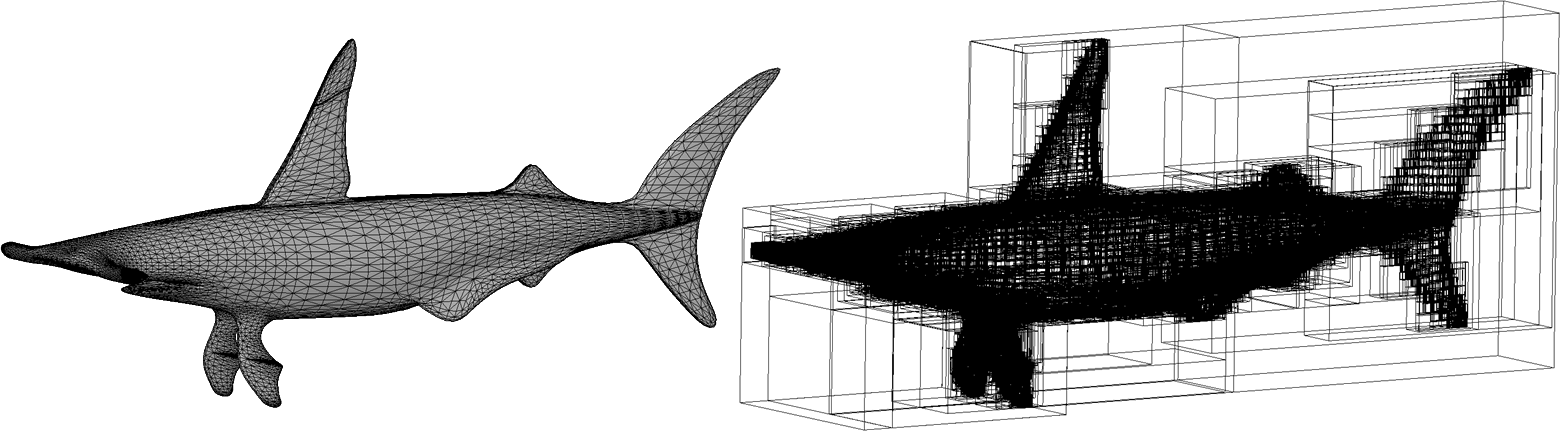
\includegraphics[width=1.0\textwidth]{AABB_tree/shark}
    \end{ccTexOnly}
    \begin{ccHtmlOnly}
        <img width="90%" border=0 src="./shark.png"><P>
    \end{ccHtmlOnly}
    \begin{figure}[h]
        \caption{AABB tree.
                 Left: surface triangle mesh of a shark.
                 Right: AABB tree constructed.}
    \end{figure}
\end{center}

% Examples
\section{Examples}
\label{AABB_tree_section_examples}

In the following example a set of 3D triangles are stored into a list. The AABB primitive wraps a triangle and an iterator in the list. We computes the number of intersections between a 3D line and the input triangles, and the closest point from a query point to the input triangles.
\ccIncludeExampleCode{AABB_tree/AABB_triangle_3_example.cpp}

The following example computes the number of intersections between a 3D ray and a set of facets of a triangle polyhedral surface. The AABB primitive wraps a facet handle and generates on the fly a 3D triangle each time its object function is called.
\ccIncludeExampleCode{AABB_tree/AABB_polyhedron_facet_example.cpp}

The following example computes the number of intersections between a 3D plane and a set of 3D segments. The segments are stored into a list, and the AABB primitive simply wraps a segment and an iterator in the list.
\ccIncludeExampleCode{AABB_tree/AABB_segment_3_example.cpp}

% Implementation Details
\section{Implementation Details}
\label{AABB_tree_section_intro}

The hierarchy construction is initialized by computing the AABB of the whole set of input primitives. All primitives are then stored along the longest axis of this box, and the primitives are separated into two equal sized sets. This procedure is applied recursively until an AABB contains conceptually only one primitive. 

In practice the design is slightly different than the one described above as the tree is leafless as presented in OPCODE \cite{opcode}. An intersection query traverses the tree by computing intersection tests only with respect to the AABBs during traversal, and with respect to the input primitives at the end of traversal, i.e., in the leafs of the tree. A projection query between, e.g., a point $q$ and a set of triangle primitives is turned into a \emph{ball} query centered at the query point. The ball then traverses the tree while recursively querying intersections with the AABBs, and computes the closest point $p$ from the query point to the input primitives only when the traversal ends at a leaf of the tree. The ball radius is then shrunk to the distance between p and q for all remaining recursive tree traversals. Efficiency is achieved through setting the initial ball radius to a small value although guaranteed to intersect the input primitives.